\subsection{Support Model}
The support models are evaluated using several metrics, including macro F1 score, accuracy, balanced accuracy, and MCC.
The results are depicted in Figure \ref{fig:support_models_metrics}.\\
From the figure, it is evident that accuracy tends to be higher than other metrics for all models,
indicating a potential bias as it overestimates model performance.\\
Among the models, the MLP ensembles generally show superior performance compared to individual models.
Notably, the MLP\_Ensemble2 model exhibits the highest performance, with a macro F1 score of 81.58 and an MCC of 81.53.
This suggests that ensemble models effectively leverage the strengths of individual models to achieve optimal performance.
\begin{figure}[h]
    \centering
    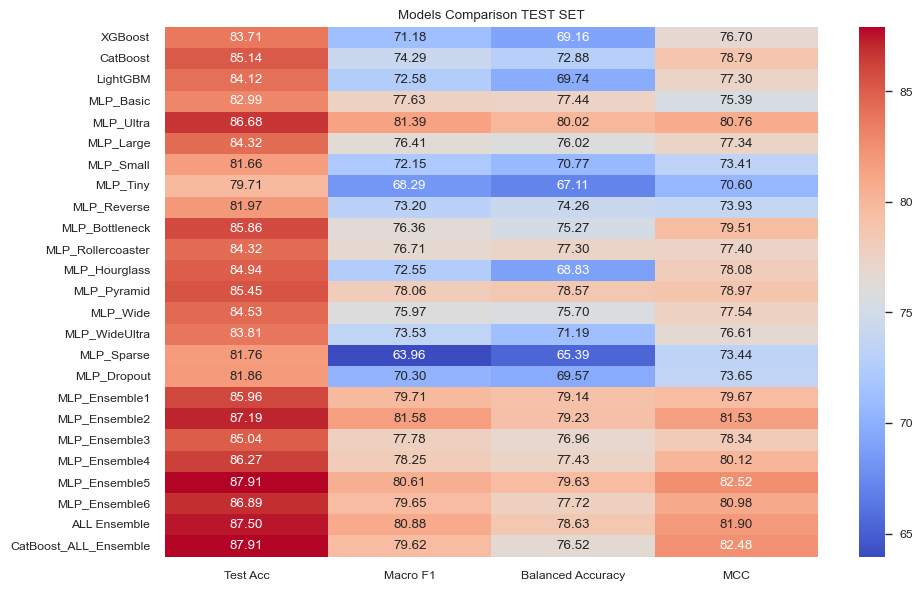
\includegraphics[width=\columnwidth]{../images/support_models_metrics.png}
    \caption{Metrics of the Support Models, computed on the test set}
    \label{fig:support_models_metrics}
\end{figure}
\noindent
The risk of misclassifying an abnormal sample as normal is depicted in Figure \ref{fig:support_models_risk_scores},
which shows the overall risk scores (in blue) for each model. The graph also displays specific risk scores associated with each class,
representing the probability of predicting a sample of that class as normal.\\
This stacked bar chart helps compare the height of the different colors rather than their areas.
From the figure, it's clear that no single model consistently outperforms others across all scores,but the performance varies across the scores.
For instance, MLP\_Rollercoaster has the best overall risk score (blue) and excels in murmurs risk score (red),
while MLP\_Ensemble3 performs best for extra systoles risk (orange).

\begin{figure}[h]
    \centering
    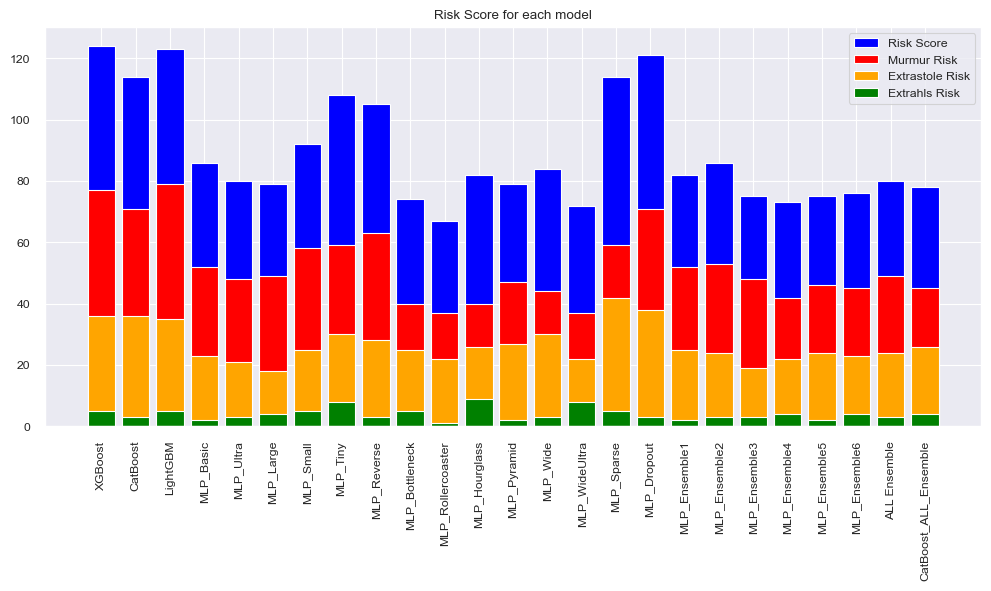
\includegraphics[width=\columnwidth]{../images/support_models_risk_scores.png}
    \caption{Risk Scores of the Support Models}
    \label{fig:support_models_risk_scores}
\end{figure}

\subsubsection*{Best Model}

The MLP\_Ensemble2 model stands out as the best-performing model among the support models.
To thoroughly understand its performance, we computed the confusion matrix on the test set, which is depicted in Figure \ref{fig:support_models_conf_matrix}.
The confusion matrix reveals that the model excels in recognizing artifacts (class 0) and extra systoles (class 1).
However, it tends to confuse murmurs (class 2) and extra systoles (class 4) with normal heartbeats (class 3).
\begin{figure}[h]
    \centering
    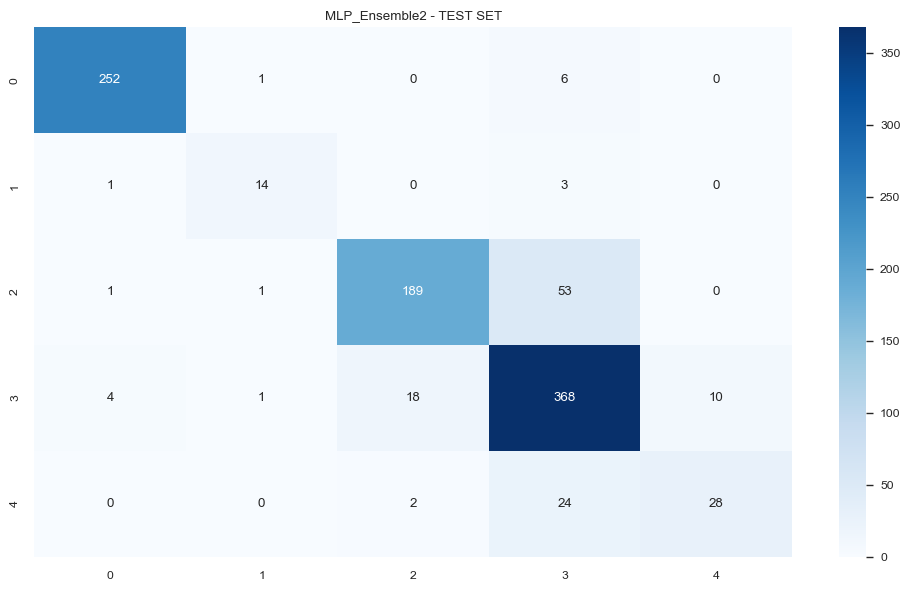
\includegraphics[width=\columnwidth]{../images/support_models_conf_matrix.png}
    \caption{Confusion Matrix of the MLP\_Ensemble2 model. Columns represent the true classes, while rows represent the predicted classes. Class 0: Artifacts, Class 1: Extra heartbeats, Class 2: Murmurs, Class 3: Normal, Class 4: Extra systoles.}
    \label{fig:support_models_conf_matrix}
\end{figure}
\noindent
To further investigate this anomaly, we analyzed the mean values of the features within each class, as shown in Figure \ref{fig:mean_val_for_features}.
The mean values represent the centroids of the classes in the feature space, providing insights into the distribution of the classes.
\begin{figure}[h]
    \centering
    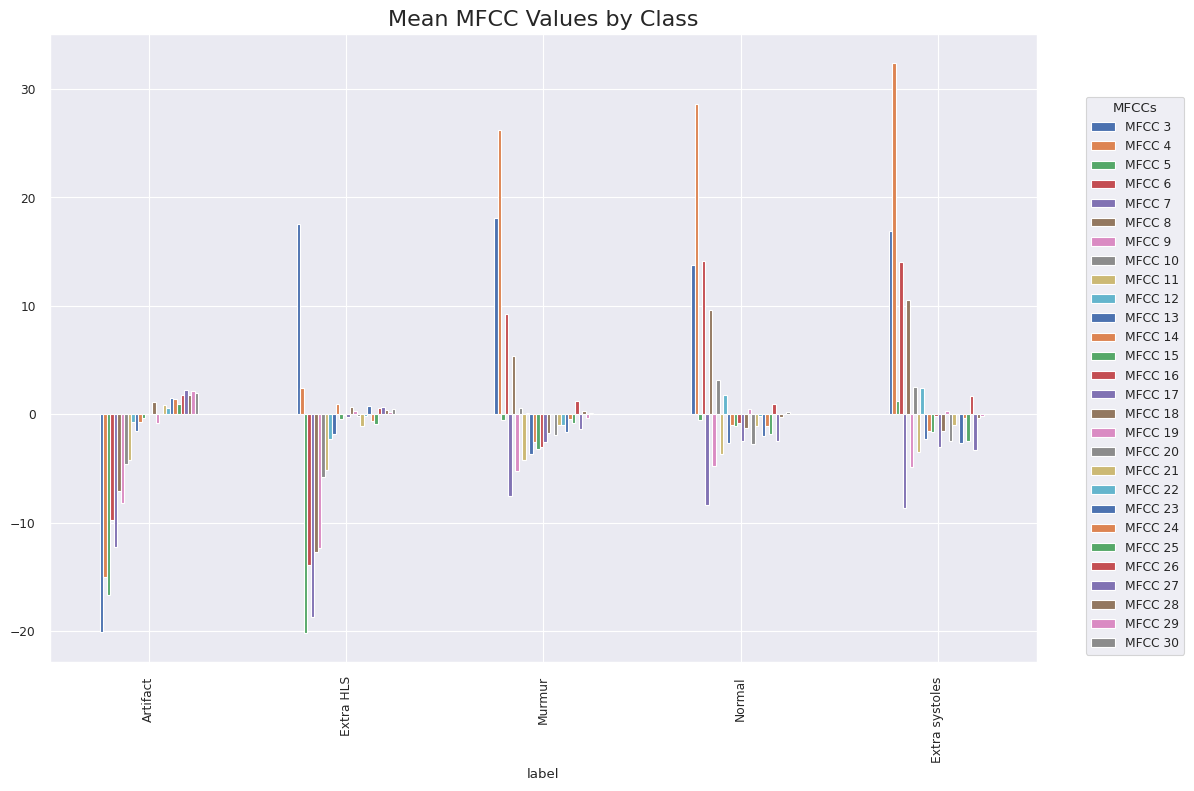
\includegraphics[width=\columnwidth]{../images/mean_val_for_features.png}
    \caption{Mean values for each feature within each class}
    \label{fig:mean_val_for_features}
\end{figure}
\noindent
The analysis indicates that artifacts and extra heartbeats have distinctly different mean values compared to other classes, while murmurs, extra systoles,
and normal heartbeats exhibit similar mean values. To visualize this better, we employed T-SNE to map the features into a 2D space, as shown in Figure \ref{fig:t_sne_visualization}.

\begin{figure}[h]
    \centering
    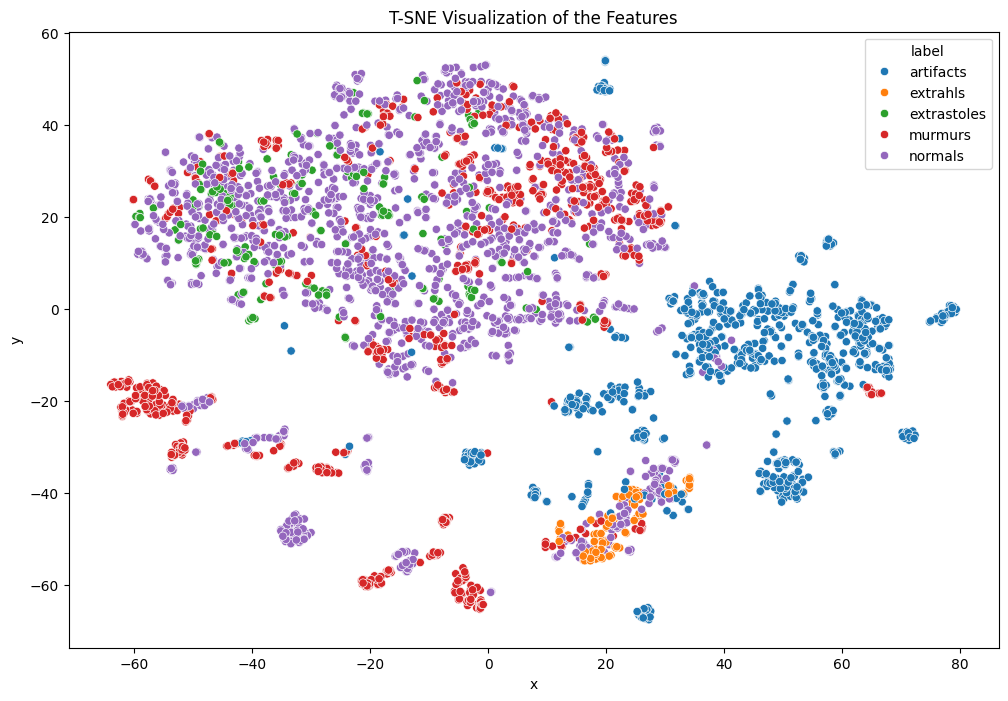
\includegraphics[width=\columnwidth]{../images/t-sne_feature_visualization.png}
    \caption{T-SNE visualization of the features}
    \label{fig:t_sne_visualization}
\end{figure}
\noindent
The T-SNE visualization confirms the clear separation between artifacts and extra heartbeats from the other classes, while murmurs, extra systoles,
and normal heartbeats are overlapped. This suggests that the features employed are not sufficiently distinct to differentiate normal heartbeats
from murmurs and extra systoles, explaining the model's tendency to confuse these classes.


\subsubsection*{Explainability}

To gain insights into the model's decision-making process, we computed the feature importance using permutation importance,
as shown in Figure \ref{fig:permutation_feature_importance}. The figure reveals that the most important features are the MFCCs, particularly MFCC 3, 4, 8, and 6.
The fact that the lower MFCCs are most important, suggest that the to distinguish between classes the model doesn't require fine details of the audio signal.
Surprisingly, the zero crossing rate and chroma features are less important, indicating that the model relies heavily on the MFCCs to make predictions.

\begin{figure}[h]
    \centering
    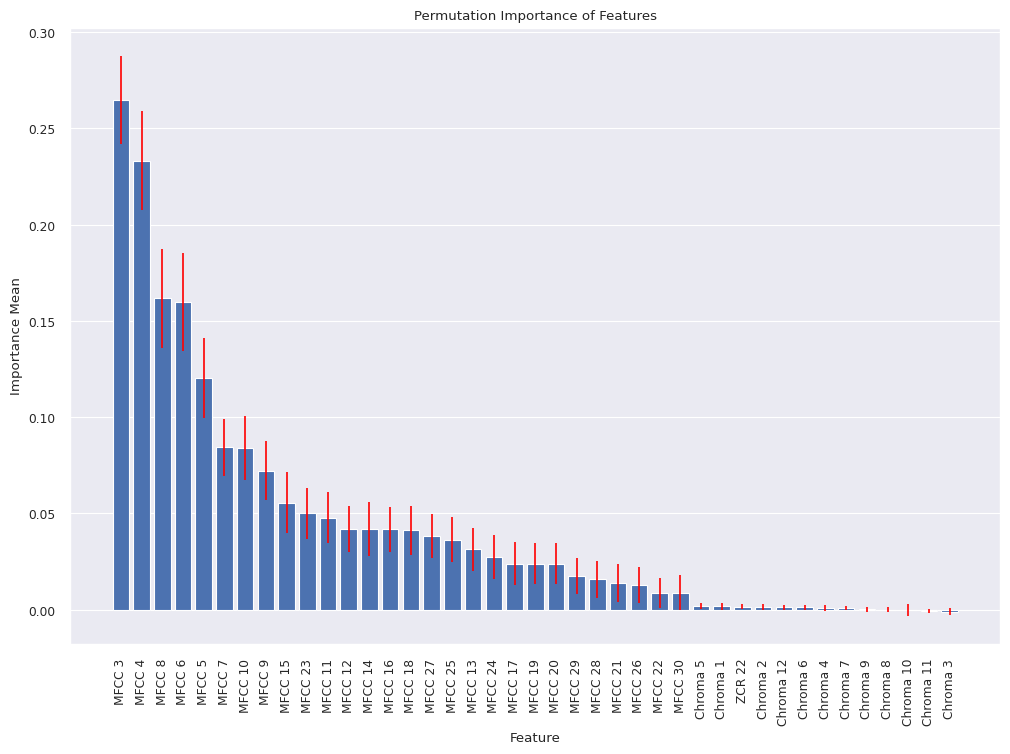
\includegraphics[width=\columnwidth]{../images/permutation_feature_importance.png}
    \caption{Feature Importance computed with Permutation Importance}
    \label{fig:permutation_feature_importance}
\end{figure}

To provide a more intuitive understanding of the model's decision-making process, especially for clinicians who may need an explanation of the model's decisions,
we identified the areas of the waveform most important for the model's prediction. This was done by first identifying the most important features
for the classification of a single sample. \\
Once the most important MFCCs were identified, we plotted the waveform of the sample along with these MFCCs.
By observing the values of the MFCCs, we can pinpoint the areas of the waveform that are critical for the model's decision.
Figures \ref{fig:extrahls_feature_importance} and \ref{fig:extrahls_waveform} illustrate this process for a single extra heartbeat sample. \\
For this sample, the most important features are MFCC 8, 6, and 3. The bar plot shows that MFCC 8 and 6 have negative values,
while MFCC 3 has a positive value, indicating that the significant areas of the waveform are where MFCC 3 is high and the others are low.

\begin{figure}[H]
    \centering
    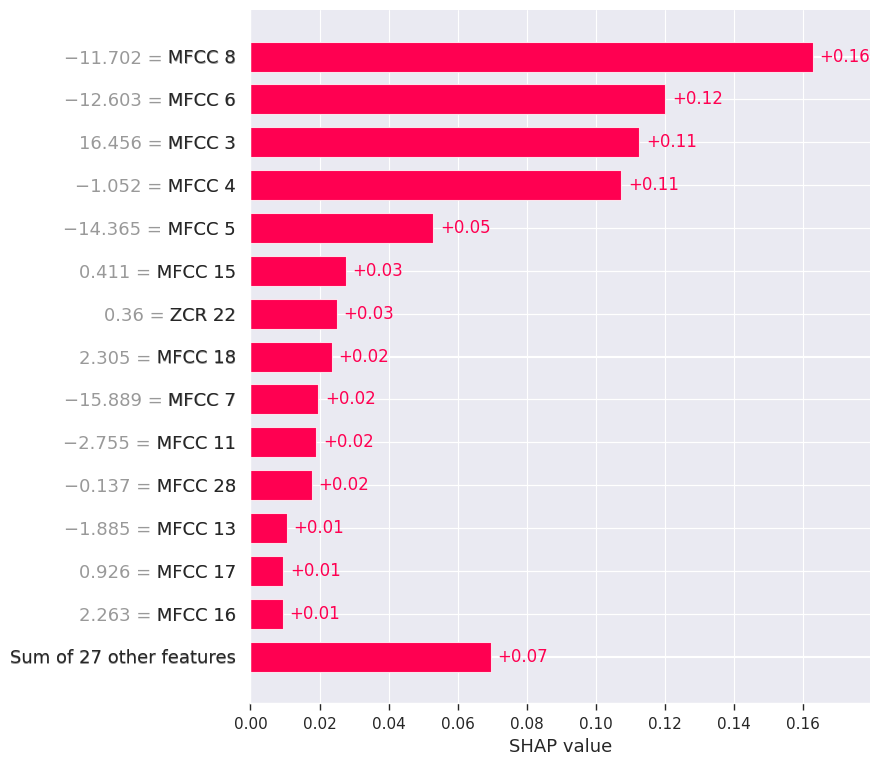
\includegraphics[width=\columnwidth]{../images/extrahls_feature_importance.png}
    \caption{Feature importance for a single extra heart beat sample}
    \label{fig:extrahls_feature_importance}
\end{figure}

\begin{figure}[H]
    \centering
    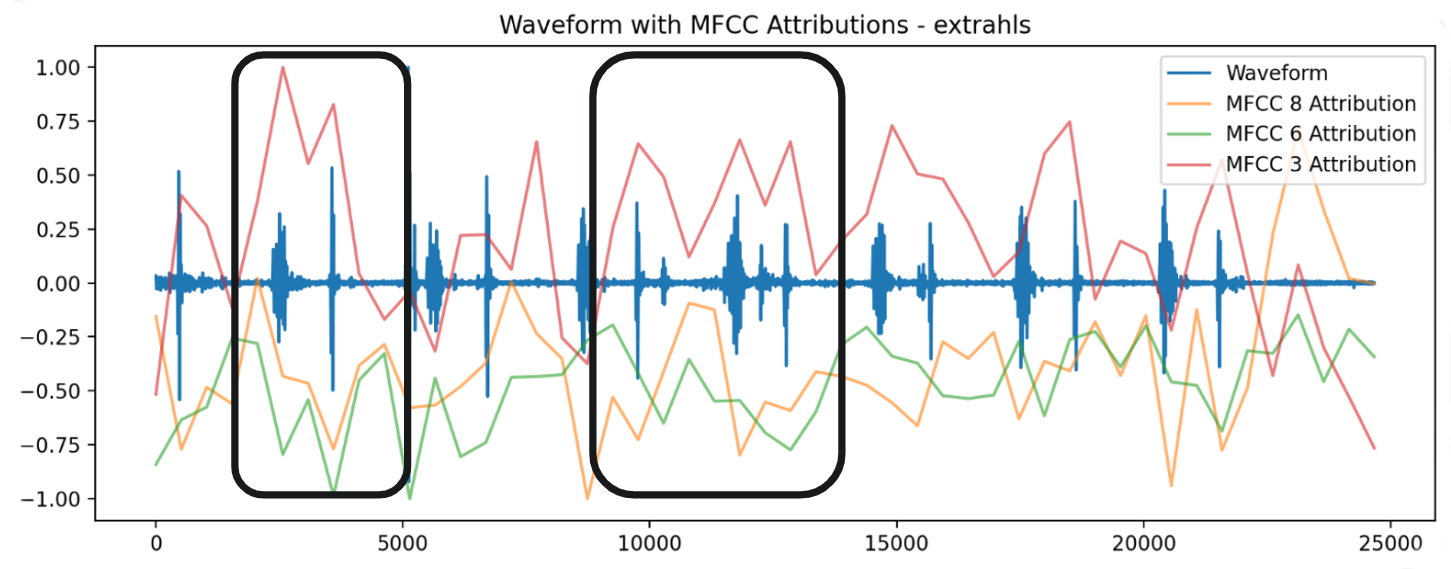
\includegraphics[width=\columnwidth]{../images/extrahls_waveform.png}
    \caption{Waveform of an extra heart beat sample, with most important MFCCs}
    \label{fig:extrahls_waveform}
\end{figure}
